\FILE{hadoop.tex}

\subsubsection{Map Reduce}

Map reduce models have been familiar to the programming and distributed
computing community for a long time and have been historically often
associated with the functional programming's map and reduce. However
the map and reduce framework introduced recently \cite{Dean:mapreduce}
distinguishes itself from such efforts while
applying it repeatedly, with fault tolerance on a very large
distributed data set. 

Instead of bringing the data to the computer in map reduce application
we often use the concept of bringing the computing to the data. This
makes a lot of sense when we assume that google has a large number of
data that is distributed an many serveres and repeated search queries
are cast to find results across them. 

In general we can define a {\em map} step, that takes the input problem and divides it
into smaller sub-problems distributing it among worker nodes. The map
function is than executed on the data distributed on the various
servers. The {\em reduce} step collects the answers of the subproblem and combines
them in some fashion. 

\begin{figure}[htb]
  \centering
    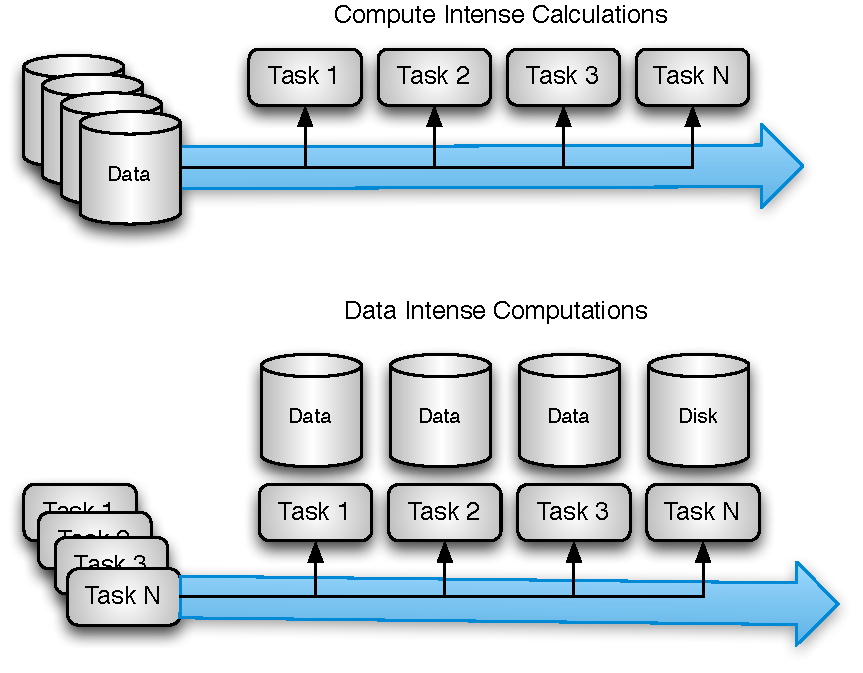
\includegraphics[width=1.0\textwidth]{images/mapreduce.pdf}
  \caption{Project Member Dist.}
\end{figure}

\paragraph{Hadoop.}\label{S:hadoop}

Hadoop \cite{report/myhadoop}\cite{myhadoop2} is an Apache project
delivering an opensource software that uses the map/reduce framework
in a distributed environment while focussing on scalability and
reliability. Its design includes the Hadoop File System (HDFS) providing an
easy to use file system to distribute the data among the servers on
which the calculations will be executed. Hadoop is designed to deal
with faults through redundancy which is an important feature when
conducting data analysis on very large distributed databases
\cite{www/hadoop}.  Hadoop is written in Java and provides the
essential map reduce functionality and allows the system to be
configured for existing hardware.

\paragraph{myHadoop.}

MyHadoop which is installed on many of the compute clusters in
FutureGrid, enables to launch Hadoop clusters via traditional
high-performance compute clusters. For this it utilizes the underlying
batch scheduling system. 

The reason for managing Hadoop jobs via a batch system may be
multiple. First, the available infrastructure is resource constrained
and utilization of disks and compute resources must be specially
accounted for to allow shared usage by many users. This naturally
happens in the educational research community quite frequently. 
Second, to efficiently utilize the compute and data infrastructure
researchers may not run Hadoop or MPI jobs continuously. At times the
may need an Hadoop environment at other time they prefer a traditional
message passing environment while at the same time being under
resource constraints.

The idea of myHadoop is to submit a job to the queuing system that
sets up a Hadoop cluster for the length of the reservation and the
researcher can than use it do conduct experiments either via
predefined jobs or in interactive mode. This is achieved by first
identifying a number of resources via the scheduler, followed by the
deployment of the Hadoop software across the identified servers. The
user will than be presented with information on how to access this
newly provisioned Hadoop cluster. myHadoop in it's new version
\cite{myhadoop2} is supported for Oracle Grid Engine (formerly known
as Sun Grid Engine), PBS, and SLURM. 

Once Hadoop has been initialized, it can be accessed through regular
job scripts as shown in Figure~\ref{F:myhadoop-script}. This example
script 8 noses are requested. It is important to set the processor per
node to 1 to assure the various Hadoop daemons are scheduled on
different servers. The rest of the script is not depicted as it
contains the actual details on setting up hadoop via the script and is
beyond the scope of this chapter. As Hadoop is a user level program, it is also
possible to run a user modified version of Hadoop which helps in
adding new features or trying out newer versions of Hadoop than the
default version that is installed for my Hadoop. The FutureGrid manual
provides more details on how to practically use myHadoop on FutureGrid
\cite{fg-manual-hadoop}.

\begin{figure}[htb]
\begin{center}
\begin{verbatim}
#!/bin/bash
#PBS -q <queue_name>
#PBS -N <job_name>
#PBS -l nodes=8:ppn=1
#PBS -o <output file>
#PBS -e <error_file>
#PBS -A <allocation>
#PBS -V
#PBS -M <user email>
#PBS -m abe

... details omitted
\end{verbatim}
\end{center}
\caption{PBS script to start hadoop}\label{F:myhadoop-script}
\end{figure}

\paragraph{Twister.}

Twister is an extension to MapReduce to allow more easily the
introduction of iterative map reduce processes. In addition twister
has introduced a number of concepts including distinction between
static and variable data, long running tasks, publish/subscriber based
communication, and varios other enhancements.  Twister is developed at
Indiana University, and is used as part of classes on distributed
systems and other educational activities. Hence it reaches popularity
within FutureGrid.

\paragraph{Virtual Clusters.} In addition to the map/reduce platforms
offered on FutureGrid, it is also possible to deploy virtual
clusters. One of the earliest such framework has been showcased by von
Laszewski while deploying a SLURM cluster. Such a cluster can than be
used as a teaching tool or provides additional mechanisms to custom
create queues and reservations. However, the most advanced feature of
FutureGrid is via cloudmesh which will allow the deployment of
clusters not only in virtual machines, but on bare metal.
